% !TEX TS-program = pdflatex
% !TEX encoding = UTF-8 Unicode

% Matthew Urffer Master Thesis
% 
% PSD Performance
%
\section{PSD Performance}

%%%%%%%%%%%%%%%%%%%%%%%%%%%%%%%%%%%%%%%%%%%%%%%%%%%%%%%%%%%%%%%%%%%%%%%%%%%%%%%
%                                                                             %
%                               PSD PERFORMANCE                               %
%                                                                             %
%%%%%%%%%%%%%%%%%%%%%%%%%%%%%%%%%%%%%%%%%%%%%%%%%%%%%%%%%%%%%%%%%%%%%%%%%%%%%%%
\subsection{PS Films}
%%%%%%%%%%%%%%%%%%%%%%%%%%%%%%%%%%%%%%%%%%%%%%%%%%%%%%%%%%%%%%%%%%%%%%%%%%%%%%%
\begin{frame}{PSD Performance (PS Films I)}
\small
\begin{itemize}
	\item Enhanced performance can be achieved with PSD (theortically)
	\item PS films show some ability for PSD
	\item None of the films are optimized \cite{zaitseva_plastic_2012}
\end{itemize}
\begin{columns}[onlytextwidth]
\begin{column}{0.30\textwidth}
	\tiny
	\begin{figure}
		\centering
		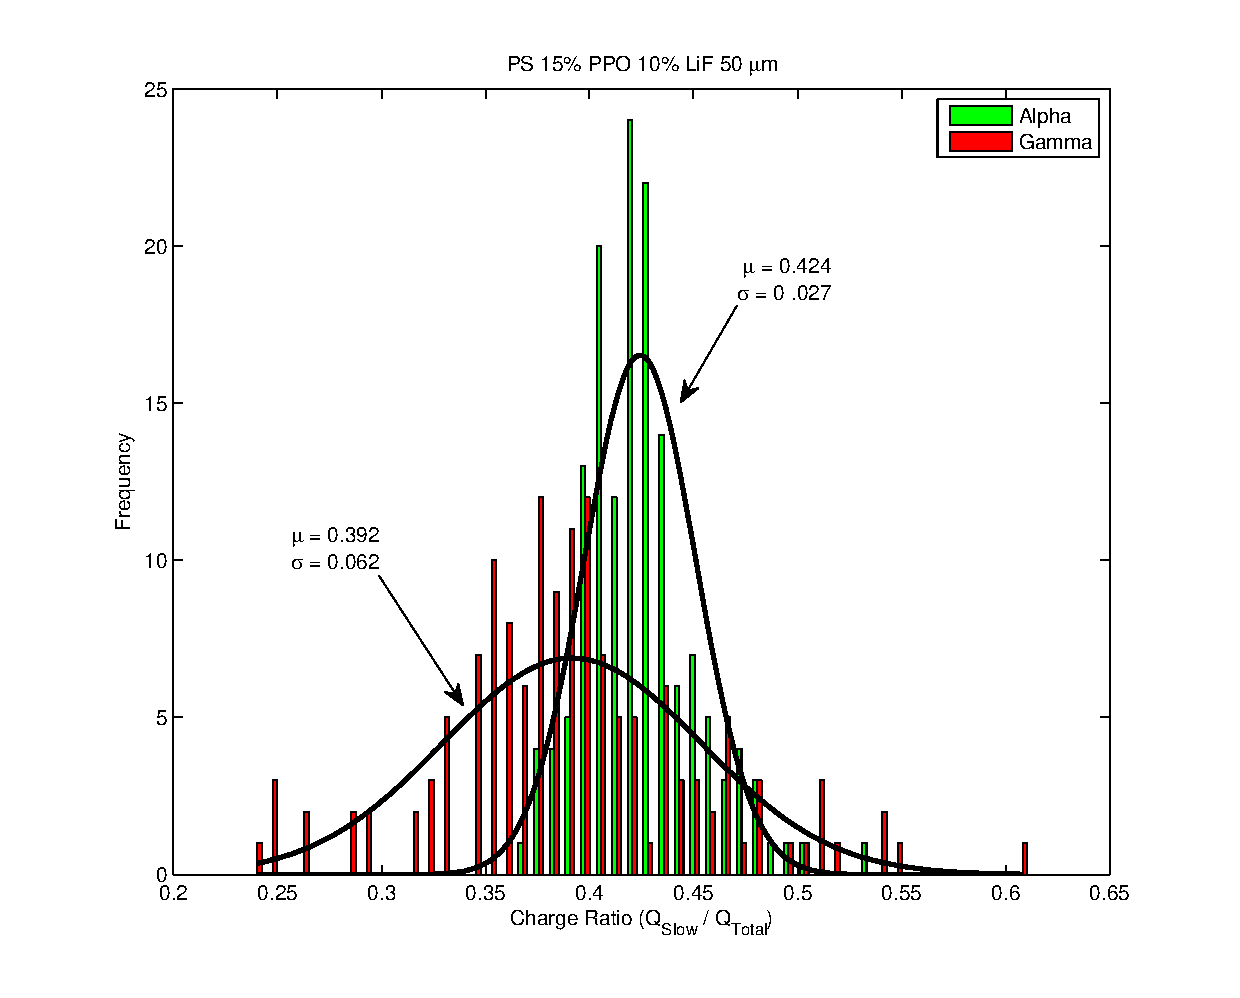
\includegraphics[width=\textwidth]{images/ChargeIntegration_PS_LiF_POP_50um.eps}
		\caption{PS 10\% LiF 50 $\mu$m}
	\end{figure}
\end{column}
\begin{column}{0.30\textwidth}
	\tiny
	\begin{figure}
		\centering
		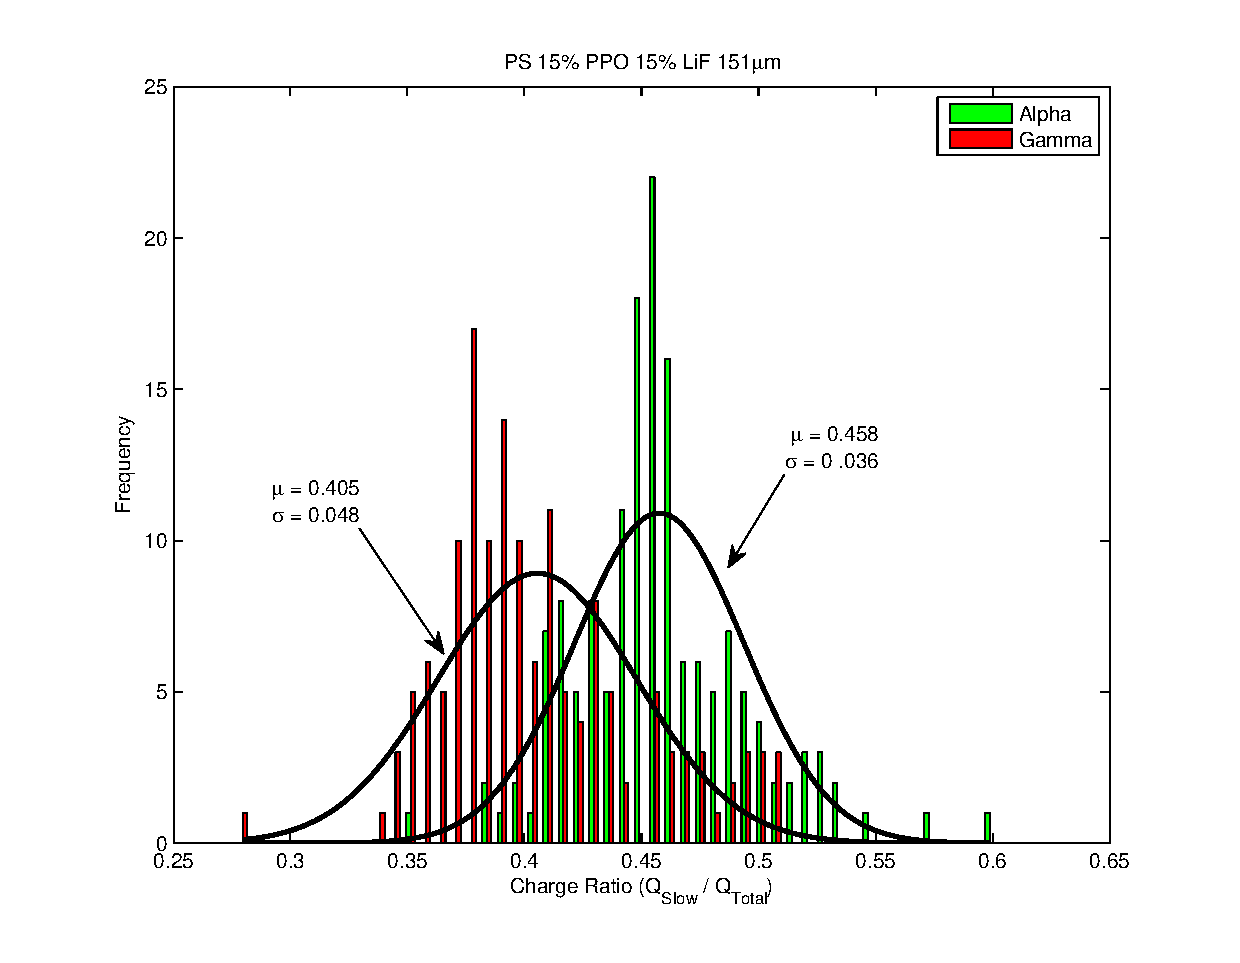
\includegraphics[width=\textwidth]{images/ChargeIntegration_PS_LiF_POP_151um.eps}
		\caption{PS 10\% LiF 150 $\mu$m}
	\end{figure}
\end{column}
\begin{column}{0.30\textwidth}
	\tiny
	\begin{figure}
		\centering
		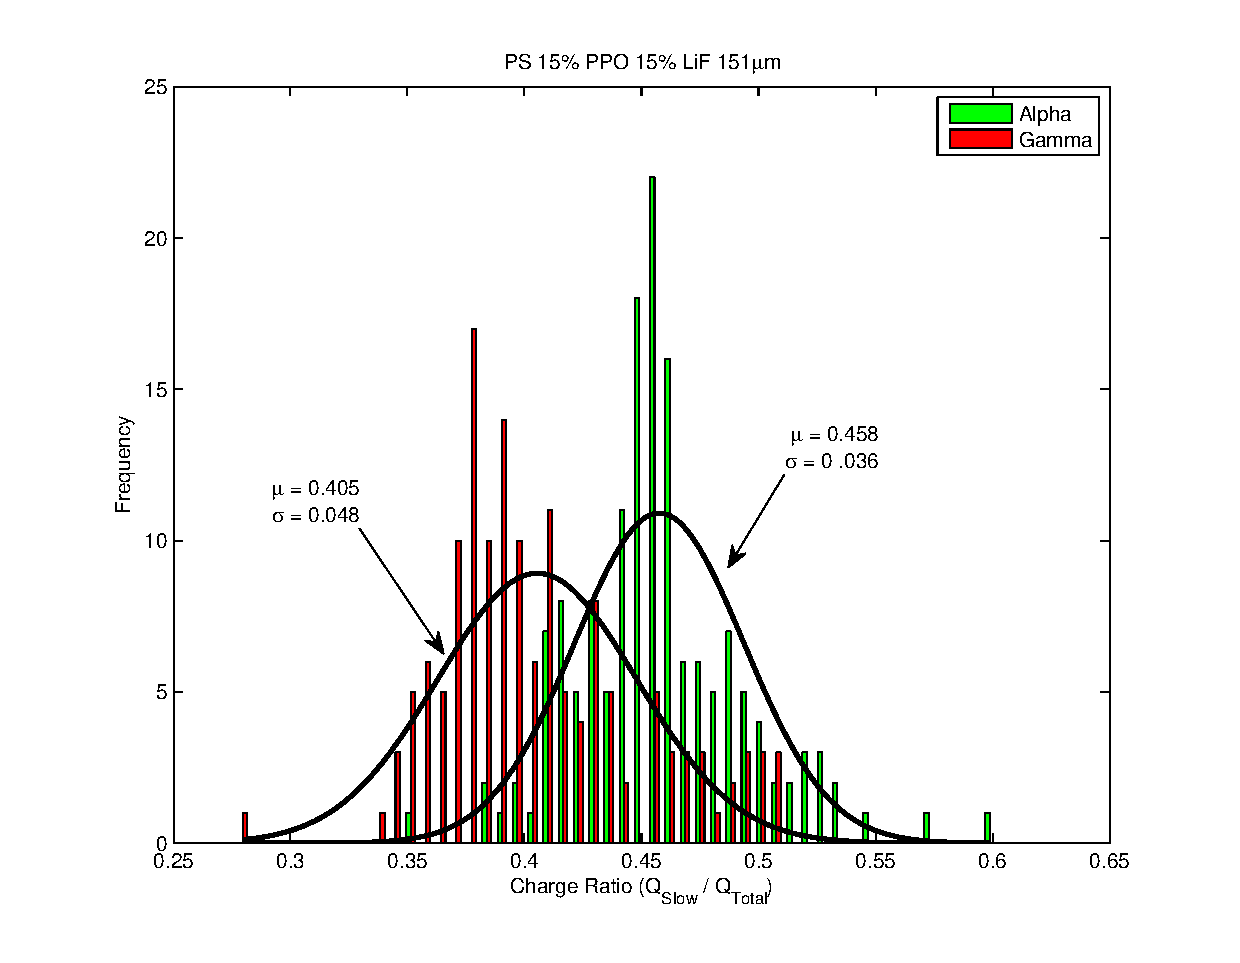
\includegraphics[width=\textwidth]{images/ChargeIntegration_PS_LiF15_POP_151um.eps}
		\caption{PS 15\% LiF 150 $\mu$m}
	\end{figure}
\end{column}
\end{columns}
\end{frame}
%%%%%%%%%%%%%%%%%%%%%%%%%%%%%%%%%%%%%%%%%%%%%%%%%%%%%%%%%%%%%%%%%%%%%%%%%%%%%%%
\begin{frame}{PSD Perfomance (PS Films II)}
\small
\begin{itemize}
	\item Thicker films tend to have better PSD
	\item Additional LiF decrease PSD performance
\end{itemize}
\begin{columns}[onlytextwidth]
\begin{column}{0.45\textwidth}
	\tiny
	\begin{figure}
		\centering
		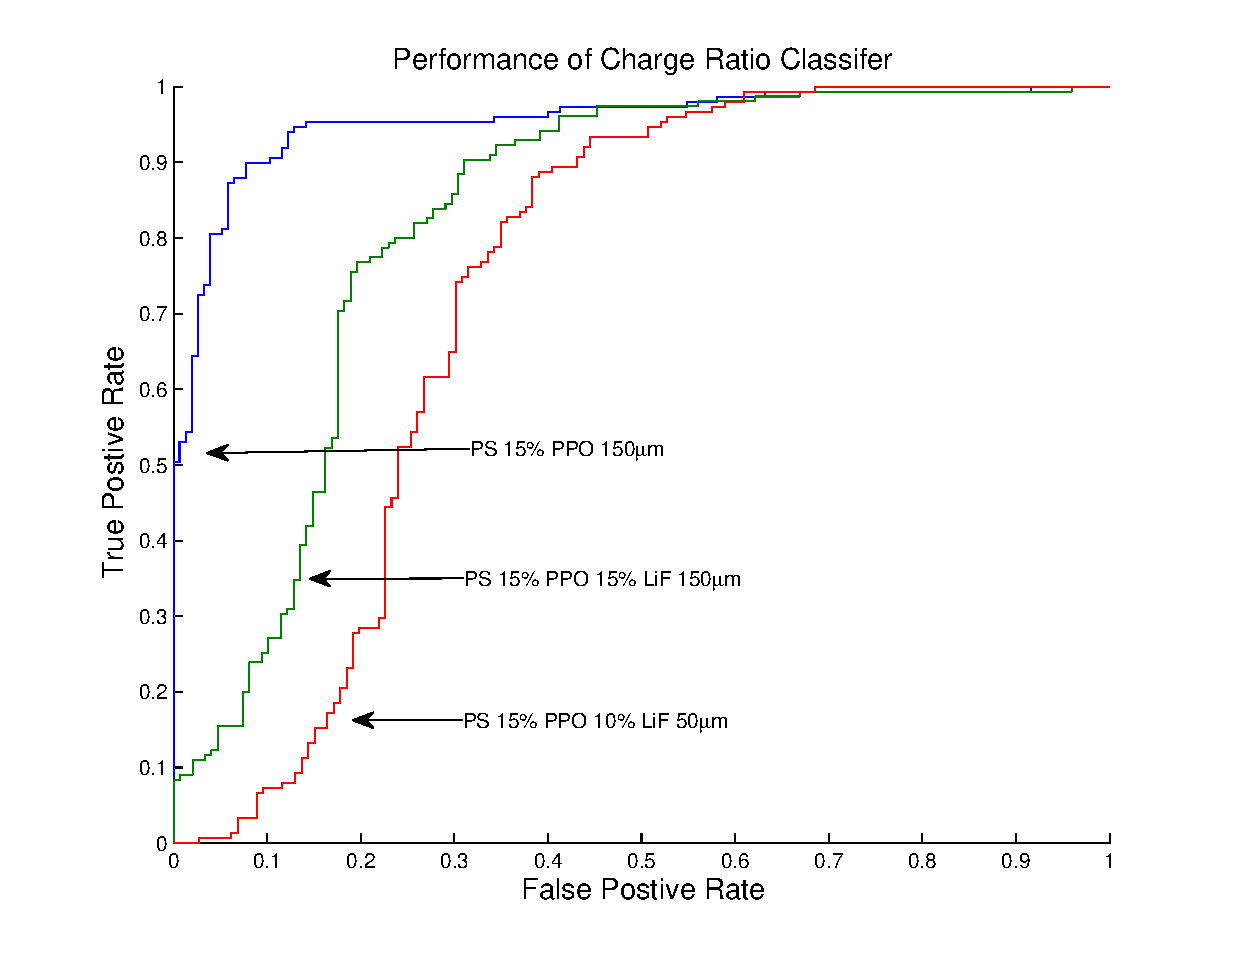
\includegraphics[width=\textwidth]{images/ROC_Comparison.eps}
		\caption{ROC Curves of Charge Intgration Classifer (PS Films)}
	\end{figure}
\end{column}
\begin{column}{0.45\textwidth}
	\tiny
	\begin{figure}
		\centering
		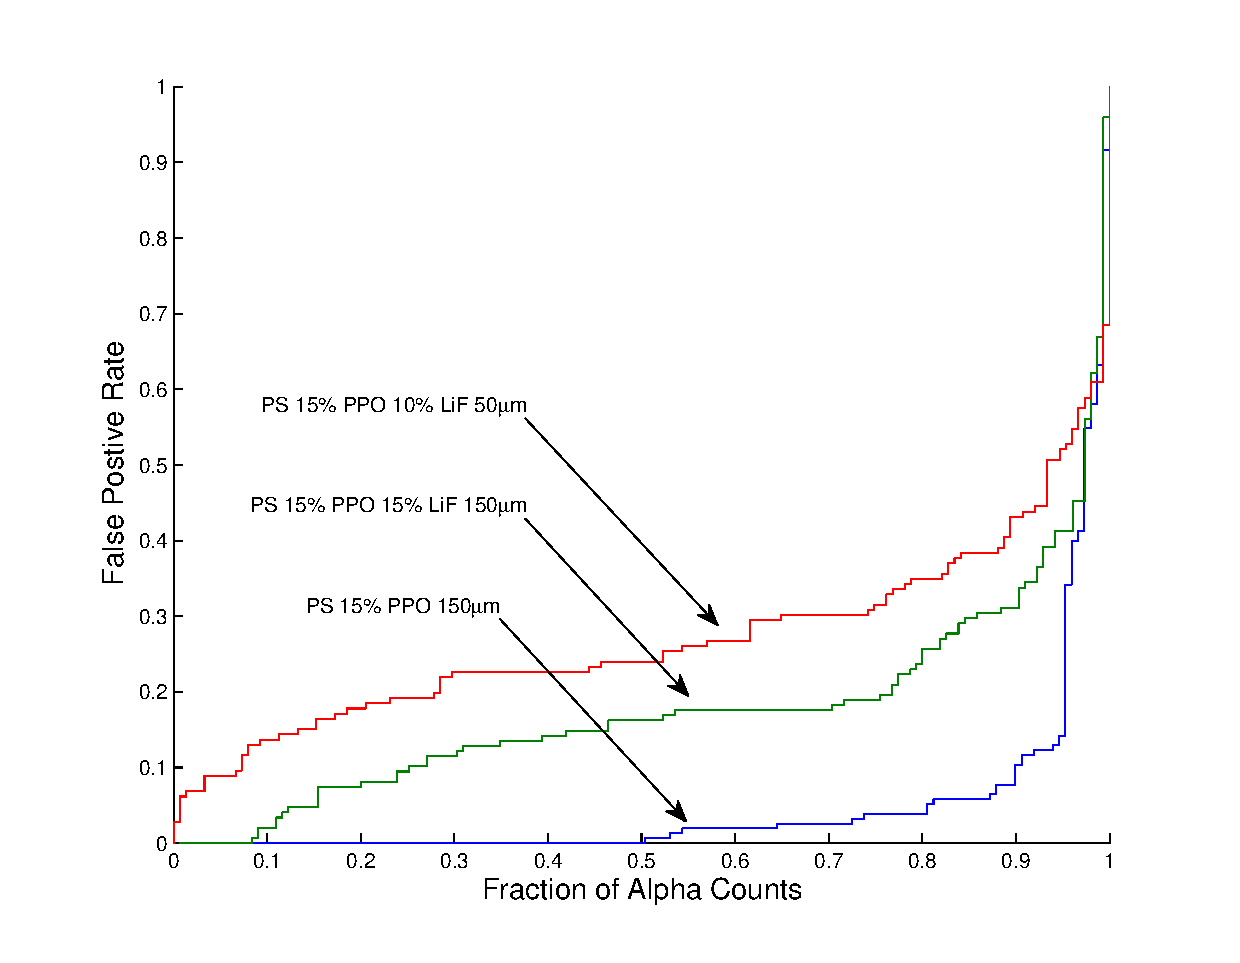
\includegraphics[width=\textwidth]{images/FPRvsFractionCounts_Comparison.eps}
		\caption{Possible Configuration}
	\end{figure}
\end{column}
\end{columns}
\end{frame}
%%%%%%%%%%%%%%%%%%%%%%%%%%%%%%%%%%%%%%%%%%%%%%%%%%%%%%%%%%%%%%%%%%%%%%%%%%%%%%%
\subsection{PEN Films}
%%%%%%%%%%%%%%%%%%%%%%%%%%%%%%%%%%%%%%%%%%%%%%%%%%%%%%%%%%%%%%%%%%%%%%%%%%%%%%%
\begin{frame}{PSD Perfomance (PEN Films)}
\small
\begin{itemize}
	\item PEN films demonstrated little capiblity for PSD
	\item PEN films where mounted on Katpon, which scintillates
	\item None of the films are optimized \cite{zaitseva_plastic_2012}
\end{itemize}
	\begin{figure}
		\centering
		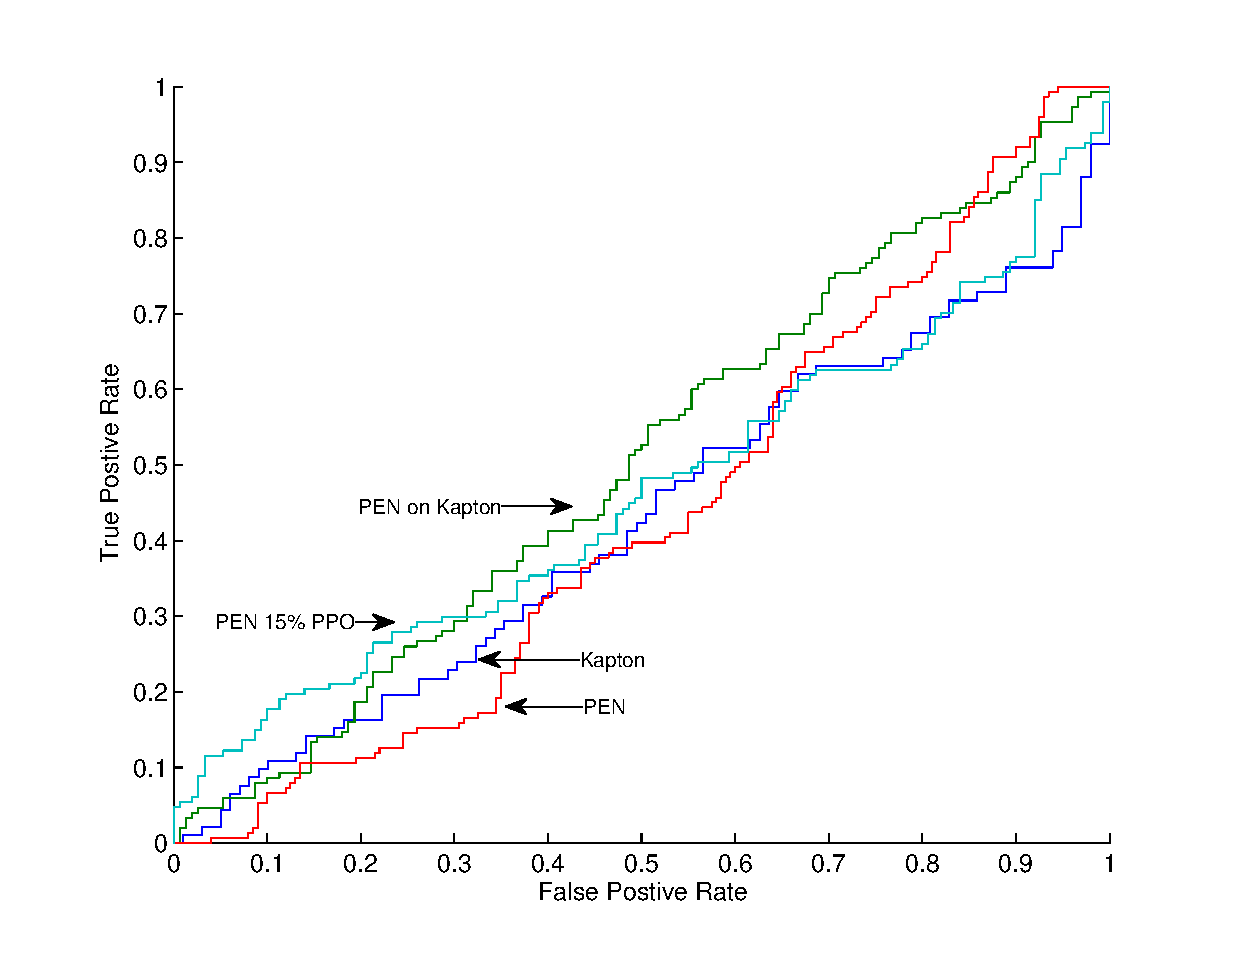
\includegraphics[height=0.55\textheight]{images/PEN_ROC_Comparison.eps}
		\caption{ROC Curves of Charge Intgration Classifer (PEN Films)}
	\end{figure}
\end{frame}
